\documentclass[tikz, border=7pt]{standalone}

\usepackage[T1]{fontenc}
\usepackage[english]{babel}
\usepackage{fourier}

\usepackage{xcolor}
\usepackage{standalone}

\usepackage{tikz}
\usetikzlibrary{shapes, arrows, shadows, calc}

\usepackage{amsmath}

\tikzstyle{data}=[
  draw,
  font=\Large,
  align=center,
  minimum height=2.5em, 
  drop shadow, 
  rounded corners
]

\begin{document}
    \begin{tikzpicture}
    	\node (model) at (0,0) {\includestandalone[mode=buildnew, width=.5\textwidth]{building_model}};
        \path (model.east) + (10,0) node[data] (geometric_features) {$v_{geom} = \begin{bmatrix}
        v_1\\v_2\\ \vdots \\ v_g
        \end{bmatrix}$};
        \path (model.south) + (4, -4) node (images) {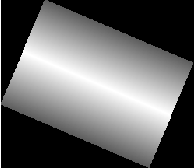
\includegraphics[width=.4\textwidth]{images/simulated_dsm}};
        
        \path (model.south) + (0, -10) node (images) {\includestandalone[mode=buildnew, width=.4\textwidth]{radiometric_input}};
        \path (geometric_features.south) + (0, -11.5) node[data] (radiometric_features) {$v_{radio} = \begin{bmatrix}
        v_1\\v_2\\ \vdots \\ v_r
        \end{bmatrix}$};
    \end{tikzpicture}
\end{document}